\documentclass[../main]{subfiles} 

% \title{Application of Differentiation 1}
% \topic{Application of Differentiation 1}
% \date{October 30 to November 3.}

% {Stewart (9E). Sections 4.1, 4.2, 4.3. Pages 280 to 309.}

\begin{document}


%--------------------------------------------------
%
% instructor notes
%
%--------------------------------------------------
Notes.
  \begin{enumerate}
    \item The topic ``curve sketching'' in Section 4.3 is postponed to next week.
  \end{enumerate}




%--------------------------------------------------
%
% learning objectives
%
%--------------------------------------------------

  At the end of the lecture, students should be able to
  \begin{itemize}
    \item identify local maximum and minimum values from the graph of a function, 
    \item identify absolute maximum and minimum values from the graph of a function,
    \item find critical numbers of a function, 
    \item apply the closed interval method to find absolute maximum and minimum values of a continuous function on a closed interval, 
    \item apply the increasing/decreasing test to find intervals on which a function is increasing/decreasing, 
    \item apply the concavity test to find intervals on which a function is concave upward or concave downward, and
    \item combine the first and the second derivative test to find local extreme values of a function, and
    \item understand the Rolle's Theorem and the Mean Value Theorem.
  \end{itemize}




%--------------------------------------------------
%
% General instructions
%
%--------------------------------------------------
% \begin{instruction}[Instruction]{How to ...}
%   \begin{enumerate}[label=(\alph*)]
%   \end{enumerate}
% \end{instruction}
%


\begin{figure}[h!]
  \centering
  \includegraphics[height=3in]{../standalones/build/plot_exercise_extreme_values}
  \caption{A grid paper for drawing.}
  \label{fig:grid}
\end{figure}

\clearpage

%--------------------------------------------------
%
% activities
%
%--------------------------------------------------
\begin{outline}{sec}{Extreme Values and Critical Numbers}{page}\label{outline:evt}
  \begin{enumerate}
    \item Let \(c\) be a number in the domain \(D\) of a function \(f\). A number \(f(c)\) is called the
      \begin{itemize}
        \item \emph{absolute maximum} value of \(f\) on \(D\) if \(f(c) \ge f(x)\) for all \(x\) in \(D\).
        \item \emph{absolute minimum} value of \(f\) on \(D\) if \(f(c) \le f(x)\) for all \(x\) in \(D\).
      \end{itemize}

      Collectively, maximum and minimum values of \(f\) are called \emph{extreme values} of \(f\). 

    \item Let \(c\) be a number in the domain \(D\) of a function \(f\). A number \(f(c)\) is called the
      \begin{itemize}
        \item \emph{local maximum} value of \(f\) if \(f(c) \ge f(x)\) when \(x\) is \emph{near} \(c\).
        \item \emph{local minimum} value of \(f\) if \(f(c) \le f(x)\) when \(x\) is \emph{near} \(c\).
      \end{itemize}

    \item (Group Activity). Make up a graph of a function over time (for example, your energy level throughout the day or the Leafs' chances of winning the Stanley Cup over time, etc.) (1) at least two local minimums, (2) at least two local maximums, and (3) one global extreme values. Make up a story about your graph by coming up with events whenever there is an extreme value. Ask a student volunteer to tell their story of the extreme values of their graph.

      A graph paper is provided in Figure~\ref{fig:grid}.
      \begin{figure}[h]
        \centering
        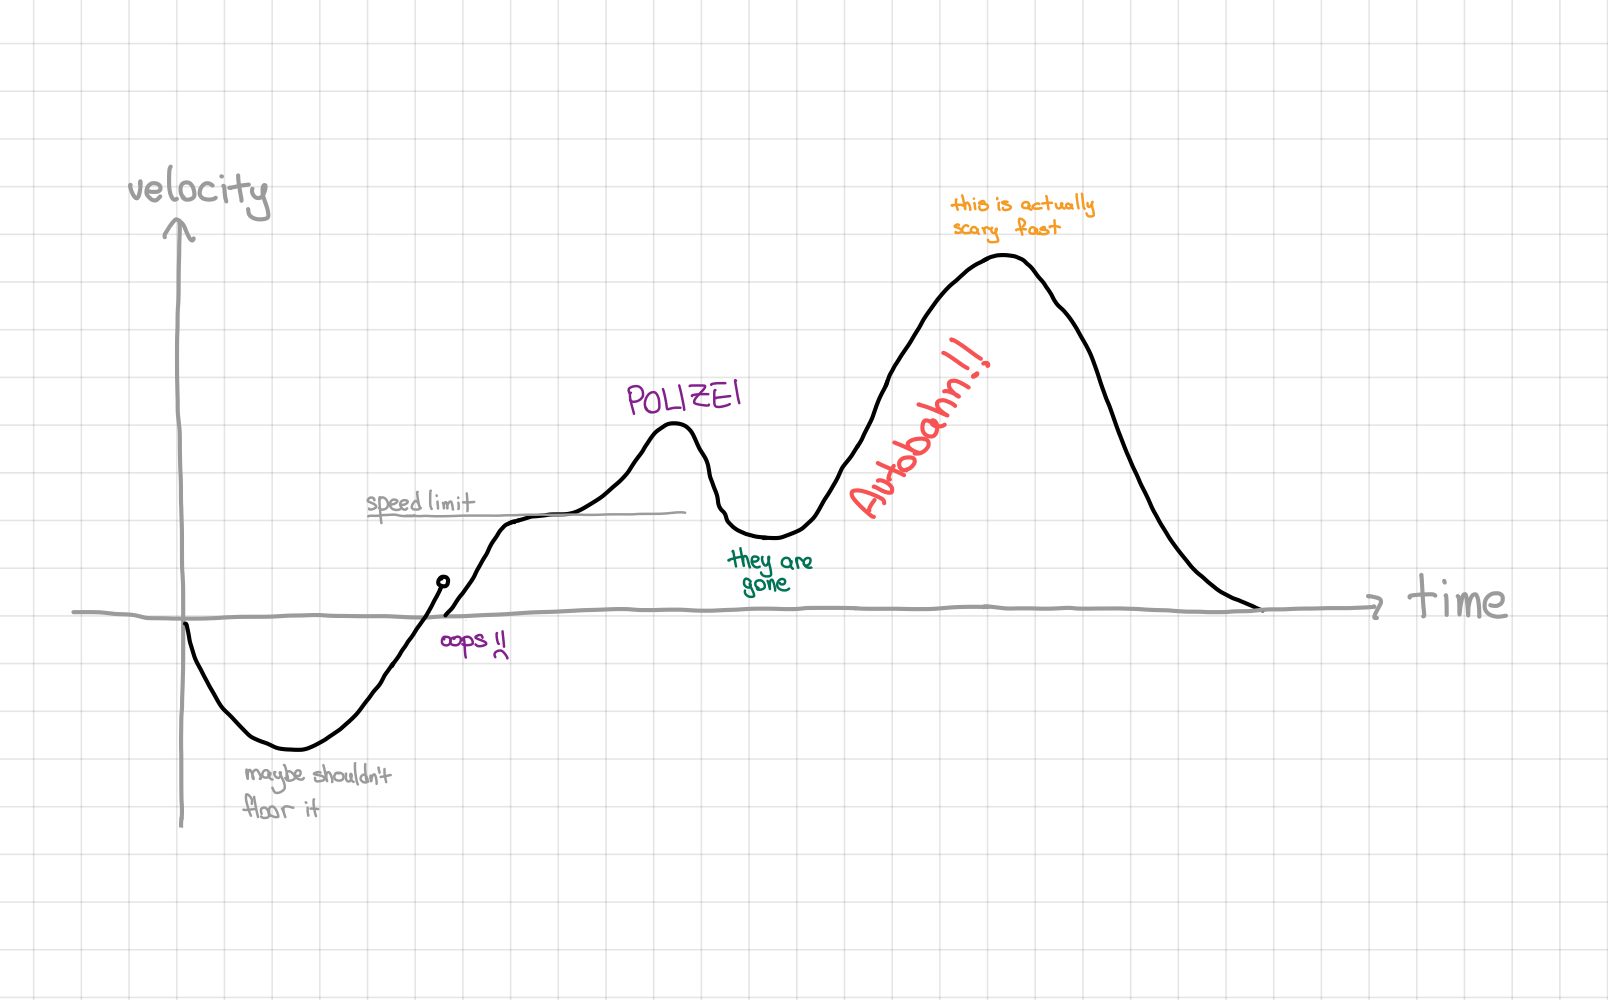
\includegraphics[width=5in]{./comic_min_max.jpeg}
        \caption{An example story of an instructor's driving.}
        \label{fig:comic_min_max}
      \end{figure}
      

    \item \textbf{Theorem} (The Extreme Value Theorem). 
      \begin{mdframed}[style=simple]
        If \(f\) is continuous on a closed interval \([a,b]\), then \(f\) attains an absolute maximum value \(f(c)\) and an absolute minimum value \(f(d)\) at some numbers \(c\) and \(d\) in \([a,b]\).
      \end{mdframed}
         
       Discuss that EVT does not give us an explicit method to find absolute extreme values. Compare this with the Intermediate Value Theorem in the textbook Section~2.5 on page 122.

     \item Discuss that the Extreme Value Theorem requires the two conditions ``\textit{continuous}'' and ``\textit{closed interval}.''  Use the functions in Figure~\ref{fig:evt_fail} to demonstrate how EVT fails when one of these requirements is not satisfied.
       \begin{figure}[h]
         \centering
           \includegraphics[width=0.3\textwidth]{../standalones/build/plot_evt_continuous_on_open}
           \quad
           \includegraphics[width=0.3\textwidth]{../standalones/build/plot_evt_discontinuous_on_closed}
           \quad
           \includegraphics[width=0.3\textwidth]{../standalones/build/plot_evt_singularity}
         \caption{Examples of functions that do not satisfy the conclusion of EVT}
         \label{fig:evt_fail}
       \end{figure}

   \item \textbf{Theorem}. 
     If a function \(f\) has a local maximum or minimum at \(c\), and if \(f'(c)\) exists, then \(f'(c) = 0\).
   \item A \emph{critical number} of a function \(f\) is a number \(c\) in the domain of \(f\) such that \(f'(c) = 0\) \emph{or} \(f'(c)\) does not exist.
   \item Explore critial numbers graphically. Use students drawings from Outline~\ref{outline:evt}. Discuss the possibility that a function can attain local or absolute minimums at more than one numbers. Similarly, discuss the possibility that a function can attain local or absolute maximums at more than one number.
   \item \textbf{The Closed Interval Method}. 

     \begin{mdframed}[style=simpleCIM]
       To find the \emph{absolute} maximum or minimum at values of a \textit{continuous} function \(f\) on a \textit{closed} interval \([a,b]\):

       \begin{enumerate}[label=Step \arabic*., start=0]
         \item Find critical numbers \(c_{1}, \dots, c_{k}\) of \(f\) in the \emph{open} interval \((a,b)\).  

           That is to find roots of the first derivative \(f'(c)\) \emph{and} wherever \(f'(c)\) is undefined.

         \item Find the values of \(f\) at critical numbers \(x_{1}, \dots, x_{k}\). 

           That is to compute \(f(c_{1}), \dots, f(c_{k})\).

         \item Find the values of \(f\) at the endpoints of the interval \([a,b]\).

           That is to compute \(f(a)\) and \(f(b)\).

         \item Compare the values \(f(a), f(c_{1}), \dots, f(c_{k}), f(b)\).
           \begin{itemize}
             \item The largest of them is the absolute maximum.
             \item The smallest of them is the absolute minimum.
           \end{itemize}
       \end{enumerate}
     \end{mdframed}
         
     
   \item Find local and absolute extreme values of the function \(f(x) = \frac{1}{3} x^3 - \frac{3}{2} x^2 + 2x\) on  \([0, \frac{5}{2} ]\).
   \item Find absolute extreme values of the function \(f(x) = x - 5\sqrt[5]{x}\) on \([-1,2]\).
   \item {For a continuous function on a closed interval \([a,b]\), extreme values can only be attained at the endpoints or at critical numbers in \((a,b)\). The Closed Interval Method takes advantage of this fact to compute extreme values on \([a,b]\).}
   \end{enumerate}
\end{outline}



\begin{outline}{sec}{The First Derivative and Increasing/Decreasing}{page}\label{outline:app_first_derivative}
  \begin{enumerate}
    \item Review the concept of \emph{increasing} and \emph{decreasing} for functions. See page 17 of the textbook.       
    \item \textbf{Theorem} (The Increasing/Decreasing Test). Assume a function \(f(x)\) is differentiable on an interval \(I\).
      \begin{mdframed}[style=simple]
        \begin{enumerate}[label=(\alph*)]
          \item If \(f'(x) > 0\) for every \(x\) in \(I\), then \(f(x)\) is increasing on \(I\).
          \item If \(f'(x) < 0\) for every \(x\) in \(I\), then \(f(x)\) is decreasing on \(I\).
        \end{enumerate}
      \end{mdframed}
         
      \begin{figure}[h]
        \includegraphics[width=0.3\textwidth]{../standalones/build/plot_increasing_decreasing}
        \quad
        \includegraphics[width=0.3\textwidth]{../standalones/build/plot_increasing_decreasing_only_derivative}
        \quad
        \includegraphics[width=0.3\textwidth]{../standalones/build/plot_increasing_decreasing_with_derivative}

        \caption{The Increasing/Decreasing Test}
        \label{fig:increasing_decreasing_test}
      \end{figure}
      \textit{Remark}. If \(f'(c) = 0\) at some number \(c\), then the function \(f(x)\) is \emph{neither} increasing \emph{nor} decreasing at \(c\).

    \item (Group Discussion) Is the Increasing/Decreasing Test useful in finding local extreme values?
    \item Determine intervals of increasing or decreasing of \href{https://www.wolframalpha.com/input?i=plot+2*x%5E3+-+9*x%5E2+%2B+12*x}{\(2x^{3} - 9 x^{2} + 12x\)}.
      \item Determine intervals of increasing or decreasing of \href{https://www.wolframalpha.com/input?i=plot+%28x-1%29%2F%28x-2%29}{\(\dfrac{x-1}{x-2}\)}.
    \item {The sign of the first derivative of a function \(f(x)\) at a number \(a\) tell us whether \(f(x)\) is increasing or decreasing at \(a\).}
    \item {The Increasing/Decreasing Test uses the first derivative of \(f(x)\) to determine whether a function is increasing or decreasing on an interval.}
  \end{enumerate}
\end{outline}



\begin{outline}{sec}{The Second Derivative and Concavity}{page}\label{outline:app_second_derivative}
  \begin{enumerate}
    \item If the graph of function \(f\) lies \emph{above} all of its tangent lines on an interval \(I\), then \(f\) is \emph{concave upward} on \(I\).
    \item If the graph of function \(f\) lies \emph{below} all of its tangent lines on an interval \(I\), then \(f\) is \emph{concave downward} on \(I\).

    \item Explore concavity graphically. See also Figure~\ref{fig:concavity}.
      \begin{figure}[h!]
        \centering
        \includegraphics[width=0.3\textwidth]{../standalones/build/plot_concave_upward}
        \quad
        \includegraphics[width=0.3\textwidth]{../standalones/build/plot_concave_downward}
        \quad
        \includegraphics[width=0.3\textwidth]{../standalones/build/plot_concave_updown}
        \caption{Examples of concave upward and concave downward functions.}
        \label{fig:concavity}
      \end{figure}
    \item \textbf{Theorem} (Concavity Test). 
      \begin{mdframed}[style=simple]
        \begin{enumerate}[label=(\alph*)]
          \item If \(f''(x) > 0\) on an interval \(I\), then the graph of \(f\) is concave upward on \(I\).
          \item If \(f''(x) < 0\) on an interval \(I\), then the graph of \(f\) is concave downward on \(I\).
        \end{enumerate}

      \end{mdframed}
        
      \begin{figure}[h!]
        \centering
        \includegraphics[width=0.3\textwidth]{../standalones/build/plot_concavity}
        \quad
        \includegraphics[width=0.3\textwidth]{../standalones/build/plot_concavity_only_derivative}
        \quad
        \includegraphics[width=0.3\textwidth]{../standalones/build/plot_concavity_with_derivative}
        \caption{The Concavity Test and inflection points.}
        \label{fig:concavity_test}
      \end{figure}

    \item A point \(P\) on a curve \(y = f(x)\) is called an \emph{inflection point} if \(f\) is continuous there and the curve changes from concave upward to concave downward \emph{or} from concave downward to concave upward at \(P\).
    \item (Group Discussion) Identify inflection points of your graph from Outline~\ref{outline:evt}. Does your inflection points correspond to real-life events?
    \item Find inflection points of the function \(f(x) = x^{4} - 4x^{3}\) and determine intervals on which \(f(x)\) are concave upward or concave downward.
    \item {The sign of the second derivative of a function \(f(x)\) at a number \(a\) tell us whether \(a\) is inside a concave upward interval or a concave downward interval of \(f(x)\). Notice the parallel to the first derivative and intervals of increasing/decreasing.}
    \item {Inflection points tell us where concavity changes in a function.}
    \item {The Concavity Test uses the second derivative of \(f(x)\) to determine whether a function is concave upward or concave downward on an interval.}
  \end{enumerate}
\end{outline}



\begin{outline}{sec}{The Derivative Tests}{page}\label{outline:derivative_tests}
  \begin{enumerate}
    \item \textbf{Theorem} (The First Derivative Test). Suppose \(c\) is a critical number of a continuous function at \(c\).
      \begin{mdframed}[style=simple]
        \begin{enumerate}[label=(\alph*)]
          \item If \(f'\) changes from positive to negative at \(c\), then \(f\) has a local maximum at \(c\).
          \item If \(f'\) changes from negative to positive at \(c\), then \(f\) has a local minimum at \(c\).
          \item If \(f'\) has the same sign on both sides of \(c\), then \(f\) has no local extreme value at \(c\).
        \end{enumerate}
      \end{mdframed}
        

    \item \textbf{Theorem} (The Second Derivative Test). Suppose \(f''\) is continuous at \(c\). 
      \begin{mdframed}[style=simple]
        \begin{enumerate}[label=(\alph*)]
          \item If \(f'(c) = 0\) and \(f''(c) > 0\), then \(f\) has a local minimum at \(c\).
          \item If \(f'(c) = 0\) and \(f''(c) < 0\), then \(f\) has a local maximum at \(c\).
        \end{enumerate}
      \end{mdframed}
        

    \item Find local extreme values of the function \(f(x) = x^{4} + 4x^{3}\).
    \item Compare these two tests.
    \item {Both derivative tests can be used to find local extreme values of a function. But the second derivative test is inconclusive when \(f''(c) = 0\) at a number \(c\) or \(f''(c)\) does not exists and we need to explore other methods to find local extreme values.}
  \end{enumerate}
\end{outline}
    



\begin{outline}{sec}{The Mean Value Theorem}{page}\label{outline:mvt}
  \begin{enumerate}
     \item (Group Discussion) If a car travelled \(200\) km in \(2\) hours, did the car reached \(100\) km/h at least once during this time?  
    \item \textbf{Theorem} (The Mean Value Theorem).
      \begin{mdframed}[style=simple]
        If a function \(f\) is continuous on a closed interval \([a,b]\) and differentiable on the open interval \((a,b)\), then there exists a number \(c\) in \((a,b)\) such that
        \begin{equation} \label{eq:mvt}
          f'(c) = \frac{f(b) - f(a)}{b - a}.
        \end{equation}
      \end{mdframed}
         
     \item By making an additional assumption \(f(a) = f(b)\) in the Meann Value Theorem, we get Rolle's Theorem. 
       \begin{mdframed}[style=simple]
         If a function \(f\) is continuous on a closed interval \([a,b]\) and differentiable on the open interval \((a,b)\) \textit{and \(f(a) = f(b)\)}, then there exists a number \(c\) in \((a,b)\) such that
         \begin{equation} \label{eq:rolle}
           f'(c) = 0.
         \end{equation}
       \end{mdframed}
         
     \item Explore Rolle's Theorem and the Mean Value Theorem graphically.
     \item It appears Rolle's Theorem is a special case of the Mean Value Theorem. But the two statements are in fact equivalent.
       \begin{enumerate}
         \item Prove Rolle's Theorem without using the Mean Value Theorem.
       \end{enumerate}
       
     \item This is also known as the Mean Value Theorem for derivatives. We will encounter the Mean Value Theorem for integrals when we discuss integrals.
     \item {The Mean Value Theorem is an existence theorem. It tells you Equation~\eqref{eq:mvt} is true for some number \(c\) but does not tell you how to find such number \(c\).}
     \item {The Rolle's Theorem is equivalent to the Mean Value Theorem. It tells you that Equation~\eqref{eq:rolle} is true but does not tell you how to find such number \(c\).}
  \end{enumerate}
\end{outline}



%--------------------------------------------------
%
% additional problems
%
%--------------------------------------------------
Exercises.
\begin{enumerate}
\item Prove the Second Derivative Test.
\item Is the constant function \(f(x) = c\), where \(c\) is some fixed number, increasing, decreasing or neither?
\item Find the interval(s) of increasing or decreasing of the function \(f(x) = x^{3}\)?
\item Prove the Mean Value Theorem from Rolle's Theorem.
\item From the textbook, exercises  1-14, 29-48, 51-67, 73-77, 80-82 in Section 4.1%Avoids curve sketching
\item From the textbook, exercises  1-18, 21-32, 37, 42,   in Section 4.2
\item From the textbook, exercises  1-21, 23-35, 40-44, 82a,b, 83-84, 88-90, 95 in Section 4.3%Is it necessary to avoid vertical asymptotes?%Some questions regarding curve sketching (45 to 68) is asked in 08_applications_2
\end{enumerate}

\end{document}

